\section{Alloy Segregation at Grain Boundary to Stabilize Polycrystalline Thin Film}
\label{Chap:Ag/ZnO:GB}


%The interactions between solute atoms and crystalline defects such as dislocations, and grain boundaries play an essential role in determining the physical, chemical and mechanical properties of solid-solution alloys. In recent years, the ability to predict solute segregation at high symmetry grain boundaries from first principles have been widely studied. However, previous algorithms have mainly focused on the simple grain boundary structures for dilute solute cases due to the costly computation power needed by density functional theory (DFT). Here, we present a general atomistic approach to optimize the structures and simulate solute segregation trends of grain boundaries in multiple component systems by the combination of a highly efficient genetic algorithm and the grand canonical ensemble, in which components are not restricted to dilute or stoichiometric cases. Different chemical potential can be used as input for creating different reservoirs for the grain boundary phases. In our study, thousands-atom grain boundary systems will be investigated by well-established empirical potentials (MEAM or EAM potentials) for Mg-based alloy systems, like Mg-Y or Mg-Zn, which are potential candidates for lightweight structural components as a result of their low density and high specific strength. Because of the complicated potential energy landscapes (PEL) coming from both geometric and occupational freedom, we will either average a good amount of small configurations by Boltzmann statistics based on their energy distributions for patterned segregation systems or use a large supercell to study cluster segregation systems across the grain boundaries. Final structures will then be used to investigate the effect of solute on mechanical behaviors of grain boundary systems.

During the heat treatment of multi-layer coating structures, quality problems like discontinuous thin films, change of colors can happen. The grain boundary grooving effect, as shown in Figure \ref{Chap:Ag/ZnO:fig15}, results in those voids and discontinuous films that degrade the quality of thin films\cite{mullins1957theory,simrick2012thermal}. This grain boundary grooving effect will increase with larger grain sizes\cite{martin2009thermal}. Therefore, we can try to stabilize grain sizes of nanocrystalline alloys by doping during heat treatment\cite{chookajorn2012design,jiao2018nanocrystalline}.


\begingroup
\begin{figure}[!ht]
  \centering
  \subfigure{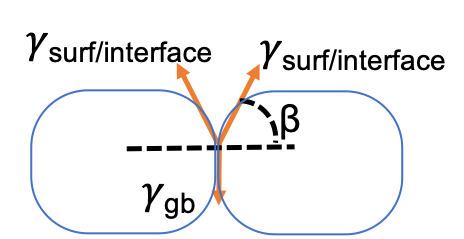
\includegraphics[width=0.65\linewidth]{Chap4/plots/Picture15.png}}
  \caption[Illustration of grain boundary grooving effects.]{Illustration of grain boundary grooving between two grains. The blue solid circle-like shape indicates two connected grains. $\gamma_{surf/interface}$, $\gamma_{gb}$ are the surface/interface energy and grain boundary energy, respectively. $\beta$ is the dihedral angle between horizon and the  $\gamma_{surf/interface}$ direction.}
  \label{Chap:Ag/ZnO:fig15}
\end{figure}
\endgroup


Solute atoms, whether they are added voluntarily for specific needs, inevitably remained as impurities after the synthesis, or introduced during the service of the material, can affect various properties of alloys by changing the stability and mobility of crystalline defects, like grain boundaries. In this section, we tried to add trace amounts of alloying elements to stabilize grain boundaries. From experiments and phenological modelling, W should segregate at Ag grain boundaries\cite{chookajorn2012design,jiao2018nanocrystalline}. We used \ac{DFT} to search for potential candidates. Simple grain boundaries like $\Sigma$5 (310), $\Sigma$3 (112) and $\Sigma$3 (111) are used. We defined the segregation energy $E_{seg}$ via,
\begin{align}
E_{seg} = E_{X near GB} - E_{X away from GB}
 \label{Chap:Ag/ZnO:eq:gb_seg}
\end{align}
where $E_{X near GB}$ and $E_{X away from GB}$ are energy when solute atoms are located close to and away from the grain boundary, respectively, for example, as shown in Figure \ref{Chap:Ag/ZnO:fig16}.


\begingroup
\begin{figure}[!ht]
  \centering
  \subfigure{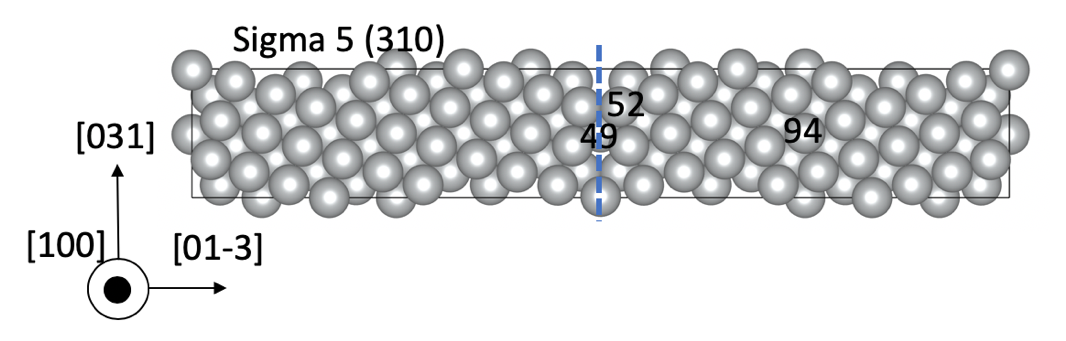
\includegraphics[width=1.0\linewidth]{Chap4/plots/Picture16.png}}
  \caption[Atomistic structure of $\Sigma$5 (310) Ag grain boundary.]{Atomistic structure of $\Sigma$5 (310) Ag grain boundary. The blue vertical line indicates where the grain boundary is. Because of a periodic boundary condition is used, there is another grain boundary at the end of the simulation box. Atom labeled with \#49, \#51 and \#94 are two atoms close to the grain boundary and far away from grain boundary, respectively.}
  \label{Chap:Ag/ZnO:fig16}
\end{figure}
\endgroup


All-electron \ac{PAW} potentials were employed for the elemental constituents with the \ac{GGA} of \ac{PBE} for the exchange-correlation energy functional, $\mu_{xc}$, and the interpolation formula of Vosko et al. \cite{vosko1980accurate}. Using plane-wave cutoff energy of at 450.0 eV, the total energy for all models of initial and final images was converged to $10^{−7}$ eV/cell. The reciprocal space of bulk supercells was sampled with (2$\times$1$\times$5), (10$\times$1$\times$4), and (5$\times$3$\times$1) k-point grids for atomic structures of $\Sigma$5 (310), $\Sigma$3 (112) and $\Sigma$3 (111). Each grid was generated using the Gamma scheme.


\begingroup
\begin{figure}[!ht]
  \centering
  \subfigure[]{
\includegraphics[width=0.49\linewidth]{Chap4/plots/Picture17a.png}}
  \subfigure[]{
\includegraphics[width=0.49\linewidth]{Chap4/plots/Picture17b.png}}
  \subfigure[]{
\includegraphics[width=0.49\linewidth]{Chap4/plots/Picture17c.png}}
\caption[Segregation energies of different elements at $\Sigma$5 (310) grain boundary.]{Segregation energies of different elements at $\Sigma$5 (310) grain boundary. The solid circles are for elements segregated at location \#49 in Figure \ref{Chap:Ag/ZnO:fig16}. And the open triangles are for elements segregated at location \#52 in Figure \ref{Chap:Ag/ZnO:fig16}. Sub-figure (a), (b), and (c) show d-elements and some p-elements in fourth, fifth, and sixth periods, respectively.}
\label{Chap:Ag/ZnO:fig17}
\end{figure}
\endgroup


A double grain boundary periodic supercell was used for constructing a $\Sigma$5 (310) grain boundary, as shown in Figure \ref{Chap:Ag/ZnO:fig16}. Atom \#49, \#52 were chosen to be atoms close to the grain boundary. And atom \#94 was chosen to be the atom far away from grain boundary. We calculated the grain boundary segregation energies for different elements in Figure \ref{Chap:Ag/ZnO:fig17}. Their segregation across the period shows a consistent trend, which is that the segregation energy increases at first and then drops. A naive explanation would be the competition between the d-electron orbital filling and the effects of the volume as atomic size increases. However, these results are contradictory to the experimental values in terms of the element tungsten(W) \cite{chookajorn2012design,jiao2018nanocrystalline}. In Figure \ref{Chap:Ag/ZnO:fig18} and \ref{Chap:Ag/ZnO:fig19}, other grain boundaries like $\Sigma$3 (112) and $\Sigma$3 (111), are also investigated using \ac{DFT}, and no case show W will segregate at either of those types of grain boundaries, despite a similar trend holds true for all of the three simple grain boundaries.

\begingroup
\begin{figure}[!ht]
  \centering
  \subfigure[]{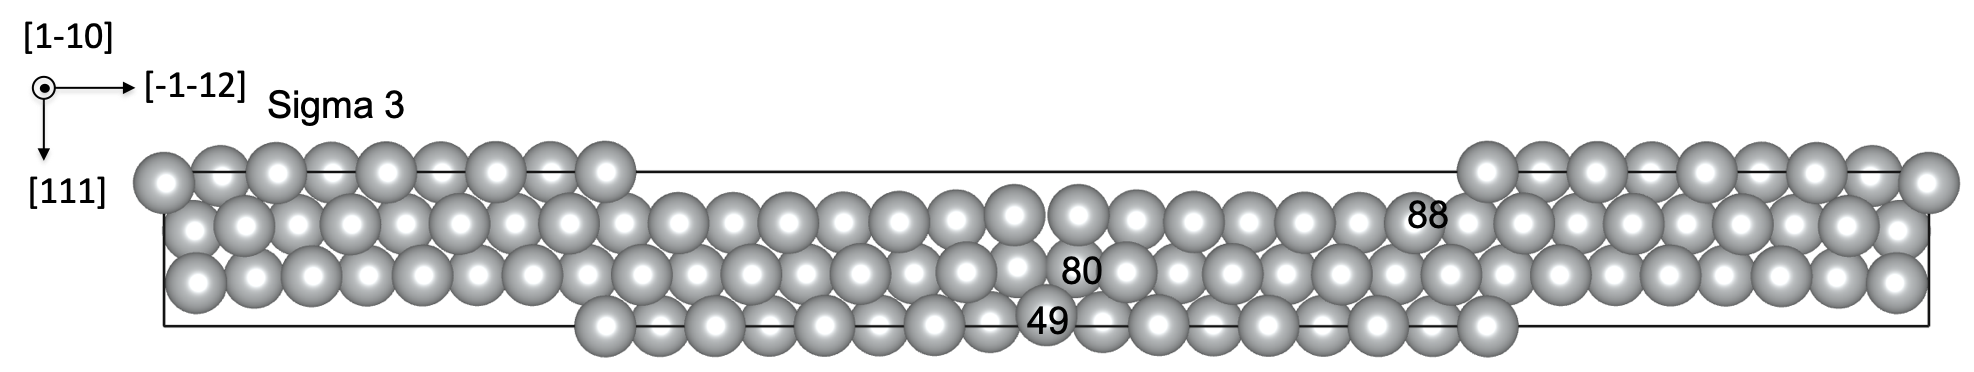
\includegraphics[width=1.0\linewidth]{Chap4/plots/Picture18.png}}
  \subfigure[]{
\includegraphics[width=0.49\linewidth]{Chap4/plots/Picture18a.png}}
  \subfigure[]{
\includegraphics[width=0.49\linewidth]{Chap4/plots/Picture18b.png}}
  \subfigure[]{
\includegraphics[width=0.49\linewidth]{Chap4/plots/Picture18c.png}}
\caption[Segregation energies of different elements at $\Sigma$3 (112) grain boundary.]{Segregation energies of different elements at $\Sigma$3 (112) grain boundary. The solid circles are for elements segregated at location \#49 in (a). And the open triangles are for elements segregated at location \#80. Sub-figure (b), (c), and (d) show d-elements and some p-elements in fourth, fifth, and sixth periods, respectively.}
\label{Chap:Ag/ZnO:fig18}
\end{figure}
\endgroup

\begingroup
\begin{figure}[!ht]
  \centering
  \subfigure[]{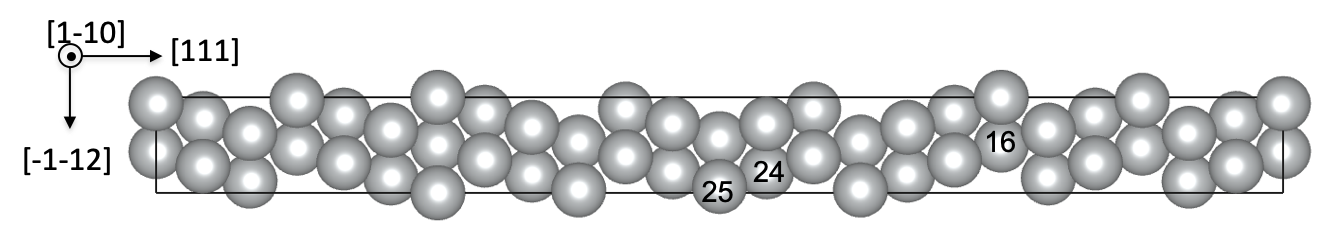
\includegraphics[width=1.0\linewidth]{Chap4/plots/Picture19.png}}
  \subfigure[]{
\includegraphics[width=0.49\linewidth]{Chap4/plots/Picture19a.png}}
  \subfigure[]{
\includegraphics[width=0.49\linewidth]{Chap4/plots/Picture19b.png}}
  \subfigure[]{
\includegraphics[width=0.49\linewidth]{Chap4/plots/Picture19c.png}}
\caption[Segregation energies of different elements at $\Sigma$3 (111) grain boundary.]{Segregation energies of different elements at $\Sigma$3 (111) grain boundary. The solid circles are for elements segregated at location \#24 in (a). And the open triangles are for elements segregated at location \#25. Sub-figure (b), (c), and (d) show d-elements and some p-elements in fourth, fifth, and sixth periods, respectively.}
\label{Chap:Ag/ZnO:fig19}
\end{figure}
\endgroup


A more complicated grain boundary, $\Sigma$29 (520), from literature \cite{zhu2018predicting} as shown in Figure \ref{Chap:Ag/ZnO:fig20}, was also studied, and it still shows repulsive interactions for W. In Table \ref{Chap:Ag/ZnO:tab3}, W segregation energy at different sites was listed. All of them show positive values except site \#196. However, when W atom was placed at that site, large distortion was observed across the grain boundary. And it was not a fair comparison to see W will segregate at that specific site \#196. Traditionally, researchers first obtained relaxed grain boundary structures from pure metals and then substitute dilute atoms to calculate alloy segregation effects. One possibility of the discrepancy we observed could be that alloying elements can not only change the chemistry of the grain boundaries but also change the atomistic structure of grain boundaries in alloys. Besides, in reality, more complicated grain boundaries, like grain boundary complexions, exist\cite{cantwell2014grain}. Therefore, more complicated grain boundary structures need to be obtained by global optimization methods, e.g. evolutionary algorithm \cite{yang2020grain}, to investigate the alloy segregation effects.


\begingroup
\begin{figure}[!ht]
  \centering
  \subfigure{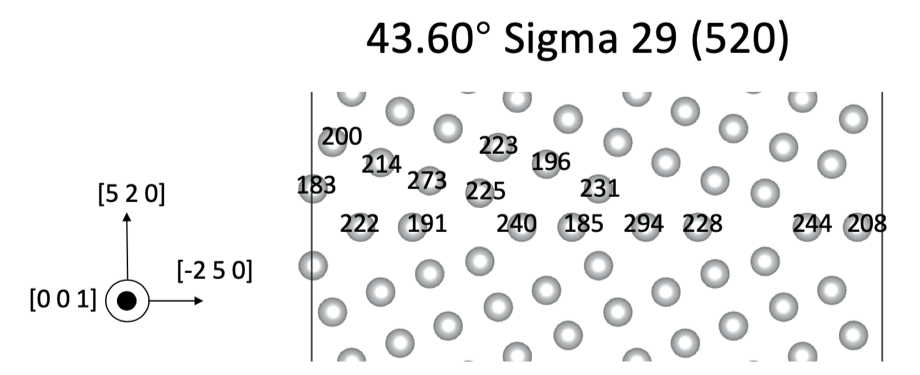
\includegraphics[width=0.8\linewidth]{Chap4/plots/Picture20.png}}
  \caption[Atomistic structure of $\Sigma$29 (520) Ag grain boundary.]{Atomistic structure of $\Sigma$29 (520) Ag grain boundary. The blue vertical line indicates where the grain boundary is.}
  \label{Chap:Ag/ZnO:fig20}
\end{figure}
\endgroup

\begin{table}[!ht]
\caption[Tungsten segregation energy $E_{seg}$ at different sites of Ag $\Sigma$29 (520) grain boundary.]{Tungsten segregation energy $E_{seg}$ at different sites of $\Sigma$29 (520) Ag grain boundary. The segregation energy $E_{seg}$ was calculated via Equation \ref{Chap:Ag/ZnO:eq:gb_seg}.}
\label{Chap:Ag/ZnO:tab3}
\centering
\begin{tabular}{cccc}
\hline
\hline
site & $E_{seg}$ eV/Atom & site & $E_{seg}$ eV/Atom\\ 
\hline
183  & .17150937     & 223  & .12724989   \\
185  & .39017180     & 225  & .26205663   \\
191  & .33935043     & 228  & .38927174   \\
196  & -.01991584    & 231  & .11203458   \\
200  & .10469391     & 240  & .51875226   \\
208  & .45059809     & 244  & .55923929   \\
214  & .02440580     & 273  & .18312458   \\
222  & .42554973     & 294  & .42944364   \\
\hline
\hline
\end{tabular}
\end{table}